99. $\cfrac{(x-5)\sqrt{x+7}}{x^6-81x^2}\geqslant0\Leftrightarrow
\cfrac{(x-5)\sqrt{x+7}}{x^2(x-3)(x+3)(x^2+9)}\geqslant0.$ Применив метод интервалов, найдём ответ: $x\in\{-7\}\cup(-3;0)\cup(0;3)\cup[5;+\infty).$
\begin{figure}[ht!]
\center{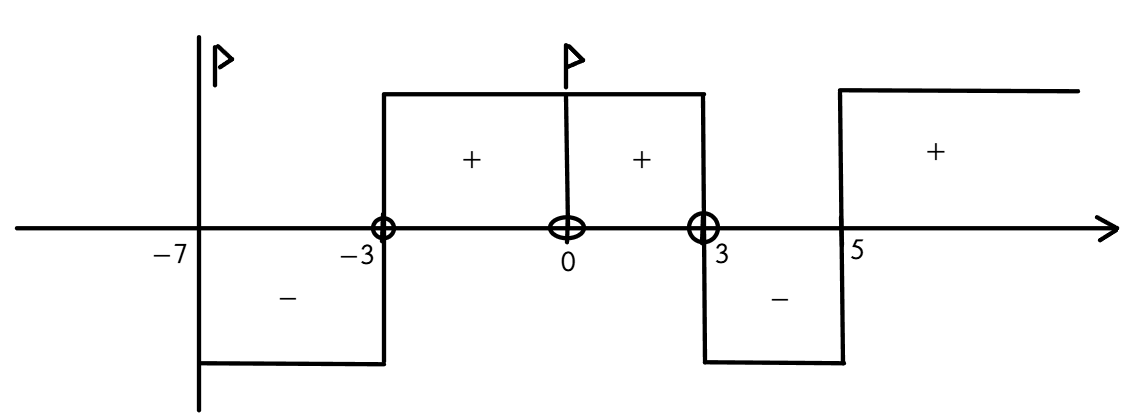
\includegraphics[scale=0.35]{int96.png}}
\end{figure}\\
